% TEMPLATE for Usenix papers, specifically to meet requirements of
%  USENIX '05
% originally a template for producing IEEE-format articles using LaTeX.
%   written by Matthew Ward, CS Department, Worcester Polytechnic Institute.
% adapted by David Beazley for his excellent SWIG paper in Proceedings,
%   Tcl 96
% turned into a smartass generic template by De Clarke, with thanks to
%   both the above pioneers
% use at your own risk.  Complaints to /dev/null.
% make it two column with no page numbering, default is 10 point

% Munged by Fred Douglis <douglis@research.att.com> 10/97 to separate
% the .sty file from the LaTeX source template, so that people can
% more easily include the .sty file into an existing document.  Also
% changed to more closely follow the style guidelines as represented
% by the Word sample file.

% Note that since 2010, USENIX does not require endnotes. If you want
% foot of page notes, don't include the endnotes package in the
% usepackage command, below.

% This version uses the latex2e styles, not the very ancient 2.09 stuff.
\documentclass[letterpaper,twocolumn,10pt]{article}
\usepackage{epsfig}
\usepackage{endnotes}
\usepackage[hyphens]{url}
\usepackage{hyperref}
\usepackage{lipsum}
\usepackage{usenix}
\usepackage{tablefootnote}
\usepackage{textcomp}
\usepackage[toc,page]{appendix}
\usepackage{titlesec}
\usepackage{enumerate}

\hypersetup{
  colorlinks=true,
  urlcolor=blue,
  citecolor=red,
}

\def\sectionautorefname{Section}

% set up tight list spacing
\usepackage{enumitem}
\setlist{nolistsep,nosep}

% for toggles
\usepackage{etoolbox}

\newcommand {\studyquote}[1]{\em ``#1''\normalfont}

% CHANGE FROM TOGGLE TRUE TO TOGGLE FALSE FOR NON-ANONYMOUS RENDERING
% http://tex.stackexchange.com/questions/5894/latex-conditional-expression
\newtoggle{anonymous}
\togglefalse{anonymous}
% \toggletrue{anonymous}

% CHANGE FROM TOGGLE TRUE TO TOGGLE FALSE TO HIDE COMMENTS
\newtoggle{comments}
\toggletrue{comments}
%\togglefalse{comments}

% Comment region command (from Wesley Willett)
\usepackage[usenames]{color}
\usepackage[usenames,dvipsnames]{xcolor}
\iftoggle{comments} {
  %if we want to show comments
  % color includes Orange, BlueGreen, NavyBlue, violet, BrickRed, OliveGreen
  \newcommand {\benzh}[1]{{\color{violet}\bf{Ben: #1}\normalfont}}
}{
  %if we don't want to show comments
  \newcommand {\benzh}[1]{}
}

%%% Local Variables:
%%% mode: latex
%%% TeX-master: t
%%% End:


\begin{document}

%don't want date printed
\date{}

%make title bold and 14 pt font (Latex default is non-bold, 16 pt)
\title{\Large \bf (Mis)perceptions of Broadband Services in Mendocino County
\\ \& How They Inform Education}

% for single author (just remove % characters)
\iftoggle{anonymous}{
  \author{
    Anonymous for submission\\
    % \affaddr{...}\\
    % \email{...}\\
  }
}{ %else
  \author {
    {\rm Nikhil Goyal, James Martin, Aishwarya Parasuram, Colin Scott, Ben
      Zhang} \\
    UC Berkeley
  }
}

\maketitle

% Use the following at camera-ready time to suppress page numbers.
% Comment it out when you first submit the paper for review.
\thispagestyle{empty}

\section{Introduction}
\label{sec:introduction}

As Yahel can attest, many users of FurtherReach wish to gain a better
understanding of the network’s technology and operational practices. Addressing
their questions has the potential to bring them both short term benefits
(e.g. satiating their curiosity, lowering operational costs for FurtherReach)
and long term benefits (e.g. enabling the community to sustain the network on
their own).


%%% Local Variables:
%%% mode: latex
%%% TeX-master: "main"
%%% End:


\section{Background}
\label{sec:background}

\subsection{Further Reach}
\label{sec:further-reach}

%% The following descriptions are from De Novo Group project description:
%% http://denovogroup.org/main/celerate-project/

The Further Reach/Celerate project is a De Novo Group~\cite{denovo} initiative
to provide affordable broadband Internet access to rural communities around the
world, thanks to a grant from Google.org and in collaboration with scientists at
Berkeley and Stanford.

Many rural communities remain disconnected or are forced to rely upon slow,
unreliable, or expensive Internet access. While many long-range networks have
been developed in the past to connect such communities, the rollouts of such
networks are fraught with complexities of both deployment and operation, leading
to higher costs and lower reliability for users. Celerate will leverage work
from the burgeoning area of Software Defined Networking (SDN) to help redefine
how such networks are built and managed.

The initial phase of Internet access rollout will begin with rural communities
in Northern California within 250 miles of the San Francisco Bay Area. This
initial rollout will enable De Novo Group and its affiliated researchers to
provide real Internet access to users while refining new approaches that improve
performance, reliability, and affordability. Beyond this initial series of
deployments, Celerate will expand to communities beyond California, and De Novo
Group will seek to partner with interested technologists around the world.

\subsection{Mendocino County}
\label{sec:mendocino-county}

Mendocino County is a county located on the north coast of the U.S. state of
California.

%%% Local Variables:
%%% mode: latex
%%% TeX-master: "main"
%%% End:

\section{Methods}
\label{sec:methods}

\begin{enumerate}
\item Analyze support tickets from Further Reach.
\item Interview Further Reach representatives (Yahel and Zean).
\item On-site in-person interview with locals.
\item Create education materials based on the interview results.
\item Distribute the materials.
\end{enumerate}

%%% Local Variables:
%%% mode: latex
%%% TeX-master: "main"
%%% End:

\section{Results}
\label{sec:results}

We first present the individual results from each method we discussed in
\autoref{sec:methods}. Then we summarize them to synthesize the final result
reports.

\subsection{Interviews with FR}
\label{sec:interviews-with-fr}

In order to understand some of the common perceptions people have regarding broadband in the Mendocino County, we decided to have an interview session with Yahel and Zean due to their on site communication expertise and their valuable experience which they have collected over the years while setting up Further Reach. Our initial goal was to determine some of the common misconceptions of people regarding broadband, which they came across while promoting Further Reach. We also wanted to gain insight into some of the common areas in Broadband which people in the County have expressed interest in learning about.

A few important aspects that we touched upon during the interview process were as follows:
\begin{itemize}
\item Some of the common questions asked by the users and the mode of communication used by them to express their concerns
\item Some of the common technical problems that have occurred in the network since its set up
\item The average education level of the local population regarding the notion of Broadband and the usage of the Internet in general
\item The techniques used by Further Reach in order to help people understand how the setup of the network works
\item Types of technical problems encountered by the users in the past and the level of detail they used to describe them
\item Queries of the users that have been difficult to solve or the users themselves had trouble understanding the explanation given to them for their concerns
\item The specific components of the network that require regular maintenance by the local technicians
\end{itemize}

From the interviews, it became evident that there were indeed some misconceptions that the local population had. While interviewing Zean, he informed us that some users are confused with the term `MB'. They don't seem to understand its usage and significance. Some users have very little knowledge about network latency and the amount of Internet speed required for different types of services such as VOIP, video streaming, email etc. He also emphasized on the need to explain to the people the difference between satellite and wireless Internet connections. From the interview session with Yahel, we came to know that some people have concerns regarding the effects of radiation from wireless networks. These concerns are of the main reasons that prevent people from signing up for high-speed Internet services. He also told us that it has been a regular practice for them to explain people about Line of Sight (LOS) and what causes its obstruction.

An important observation that both of them made was that most of the people within the Further Reach network are quite aware of the importance of broadband and the various services and usages it comes with. Thus the education material that we would prepare should aim towards the population who do not have access to high-speed internet access nor any ways to gain information about it

\subsection{Support Tickets Analysis}
\label{sec:supp-tick-analys}

In order to reduce the scope of our research problem, we first decided to identify some of the common types of concerns and queries that people have when they have already been provided with high-speed Internet connection. For this, we used the ticketing system used by Further Reach’s team for tracking its customer’s questions. We analyzed over 1425 tickets filed since August 2014, each depicting a particular customer’s query or concern. Based on our analysis, we identified 9 major categories of concern:

%% See the end of this file:
%% https://docs.google.com/document/d/1LdyNFUBUV0URWayc8kXM2SXaAhWg2FWJO2_8w2IgTvU/edit

\begin{itemize}
\item \textbf{Payment.} This category included tickets filed by the people who had specific problems or general questions regarding paying online bills. Some common problems were error in billing transaction, autopay not correctly set up, inability to understand the online payment system’s GUI etc.
\item \textbf{Subscription Requests.} Many asking for the service. Some offer new relay
  sites or act as local tech volunteer, in areas like Albion and Gualala. % though locations aren't good
\item \textbf{Quality of Service.} This category included concerns in which people expressed dissatisfaction with the service/plan they were paying for. 
The main concern given was high cost but slow Internet speed or poor Internet
connectivity. Many users attempted to run SpeedTests to make their point.
\item \textbf{Troubleshooting.} Antenna not installed? System down? Many people call
  about the internet being down. A large number of reasons ranging from extremely ambiguous to highly specific were given for system outages.
\item \textbf{Questions about Equipment.} In this category, people asked help for assistance in set up/installation and maintenance of equipment provided to them by Further Reach in order to help them gain access to the network
\item \textbf{Interference with other Wireless.} There were a few tickets which claimed
that they were receiving poor signal strength due to interference with other
wireless networks within the area, e.g. AT\&T towers.
\item \textbf{Requests for unusual features.} Many tickets asked for availability of various types of internet services that are available with the download/upload speed the users signed up for such VOIP features, streaming videos using Netflix, paying bills online etc.
\item \textbf{Passwords.} Several tickets provided the SSID/password of their
network and hoped that a technician could solve the connection issue.
\item \textbf{Alternate Pricing.} Tickets in this category asked for details about
Internet plans other than the one the corresponding user had, for example
vacation prices and discounts, non-profits requesting free service, etc.
\end{itemize}

The above categories played a pivotal role in helping us formulate interview questions that mainly target the concerns of the population living outside the Further Reach network regarding high-speed Internet connection.

Essentially, when we analysed the level of detail provided about the problem
at hand in each ticket, it helped us understand the average level of knowledge
the users had regarding broadband. We also learnt about some of common
difficulties users face while accessing various internet services, one of them
being trouble with paying online bills. Some tickets also helped us understand
the main concerns people have with wireless internet access. These included
vulnerability to EMF from electronic devices and the health problems
associated with it. Based on the locations of the users filling the tickets,
we were also able to get an insight into their interest in high speed internet
access. This helped us decide on locations outside the Further Reach network
where we could conduct on site interviews and try to understand what hold
people back from signing up for high speed internet access. 

\subsection{Interviews with Rural Residents}
\label{sec:interv-with-rural}

With the help of Mendocino Community Network (MCN), we recruited 
residents from Mendocino County using a flyer that was put on public display and distributed.
Of the number of residents who expressed interest in the survey, we were able to interview
nine residents, 5 in person and 4 over the phone. The residents were selected among those
who did not currently have FurtherReach. All of the residents were asked for interviews
already had internet access through another provider.

Based on our ticket analysis and interview sessions with Yahel and Zean, we consolidated a list of interview 
questions that touched upon the various categories identified in the trouble tickets section. While preparing
the questions, we tried to avoid the assumptions that are our interviewees would have some considerable level 
of knowledge about broadband and the services it offers. We also tried to make sure that none of our questions
make the interviewees feel uncomfortable while responding. Table~\ref{tab:questions} lists the questions
we prepared.

The questions were meant for
them to express their opinions as openly as possible with as little bias introduced by the
phrasing of the question or our opinions. We, being all engineering-oriented,
were biased toward the use of technology and may have introduced some bias. In addition
to the interviewee's personal opinion, he or she was also asked about the opinions of her
neighbors.

\begin{table}
\begin{enumerate}
    \item What does broadband mean to you?
    \item Do you have any concerns of high speed? Some part you don’t understand?
    \item Any concerns about health/safety?
    \item Incase we put a tower close to your house, what specific concerns u would have?
    \item Incase you are provided with high speed internet connection, what would you mainly use it for?
    \item What is a reasonable price range for high speed internet in your opinion?
    \item What degree of awareness do you have about the difference between various technology?
    \item Your relatives usage of network and their concerns?
    \item Is there something holding people from signing up for network?
    \item Do you use any specific software to test speed of network?
    \item How many people do you think would be interested in a better broadband service in a 10 mile radius?
    \item How comfortable are you while paying bills online?
    \item Have you considered internet as substitute for TV~?
    \item Have you contacted Further Reach to setup a network?
    \item What was your reason to participate in the interview?
    \item Do you participate in netbanking or shopping online?
    \item Do you think internet will be useful for kids
    \item What would you think is most imp that should be included in our educational material? And how would we distribute them?
    \item What is your present internet provider and how much are you currently paying?
    \item Any negative perception of broadband?
    \item What is your current speed?
    \item What would you think you can do with Internet but you don’t know how to do?
    \item Different people’s experience? Line of sight point of view?
    \item Do you have a sense what the younger generation would do with broadband, which they can’t do now?
\end{enumerate}
\caption{Interview Questions}
\label{tab:questions} 
\end{table}

All of the residents that were interviewed expressed an interest in broadband and bringing it
to the Mendocino County. Unfortunately, there were no residents who asked to be interviewed who 
were of the opinion that broadband should not be present in Mendocino. In addition, 44.4~\% of
the interviews were considered technically knowledgeable by us.

Aside from the desire to have broadband made available to the homes, the opinions of the 
interviewees varied. Many did express some concern for the radiation emitted by antennas
used for wireless internet access. However, their concerns were not enough to prevent them
from using WiFi at home or from using FurtherReach if it were to be made available.
Most interviewed residents were more concerned about the aesthetics of an antenna on his or her
house more than the potential hazard of the RF radiation.
There was a belief that there were those in the community who had major concerns about radiation
from RF antennas. However, these individuals who had major concerns of radiation were described
as being a small minority who had little effect on policy making in the community.

Although many of the residents interviewed described were technically knowledgeable, they felt
that it would be valuable for their community to have technology education made available such
as technology centers for this purpose. Some interviewees also felt that education at the school
for children would be valuable. These same interviewees also described having broadband available
as being most beneficial to the younger population for educational purposes.

There was a technical concern from many residents who felt that wireless broadband by use of
line-of-sight would be infeasible given the terrain that surrounds the house. However, based
on the addresses of these residents and what the residents described, we felt
that it would be technically possible to deliver wireless internet. However, the cost of
installation was not evaluated.

Cost of installation was a major factor for their choice of internet access presently. Broadband
through the use of fiber is available to the home. There is currently fiber deployed on many
streets in the area. However, the cost of installation of the fiber has been quoted to be at least \$2000.
Most residents felt this cost was too high if they must also pay for a very high regularly monthly bill, all
estimates exceeding \$100. Residents are currently paying for internet access between \$50--\$200
through technologies such as satellite or other line-of-sight providers.

Most residents seem to be knowledgeable as to the difference between broadband access and slower speed internet.
However, there were some confusions that were concerned with some of the details. One often confused topic was
the difference between bandwidth in terms of throughput and a regular bandwidth cap. Another confusion was
as to the bandwidth caps present in cellular services that have no perceived bandwidth cap and the fact that
customers are rate-limited if too much data is used. Lastly, some residents were unclear as to the differences
between the wireless implementations of satellite and terrestrial and its effect on quality of service.

Due to the small sample size of an area of a small number of people,
we chose not to publish some of the details of some of the
interviews for reasons of privacy.


%%% Local Variables:
%%% mode: latex
%%% TeX-master: "main"
%%% End:

\section{Education Materials}
\label{sec:education-materials}

\benzh{Show our results. Either excerpt of texts; or figures, screenshots of
  websites.}

%%% Local Variables:
%%% mode: latex
%%% TeX-master: "main"
%%% End:

\section{Lessons Learned}
\label{sec:lessons}

As computer scientists who have never been trained in how to conduct qualitative
research, this project was an excellent learning
experience for us. Here are a few lessons we learned along the way:

\begin{itemize}
\item Broadly speaking, qualitative research is really difficult! It is time
consuming and challenging to come up with interview questions that really
focus on the key issues without biasing the responses. Moreover, conducting
interviews is challenging itself, and thoroughly synthesizing the results of
the interviews more-so.
\item It is highly challenging (if not impossible!) to conduct interviews in a
non-biased way. We often walked away from interviews wishing that we could do
them over again, because we felt that the way we had phrased the questions in
a way that primed the interviewee to respond in a particular way. A general
takeaway from this is that we should strive to ask questions in a way that
gets interviewees to do most of the talking, where they can frame issues in
their own words.
\item Snowball sampling seems like a great idea. Sampling bias was pervasive in our interviews; most of our
interviewees were pro-broadband, and we did not manage to find many
anti-broadband viewpoints,
or people who could not afford broadband. This was largely an artifact of the
way that we distributed our request for interviews: having Shirley (MCBA)
email a mailing list of people who are likely actively tuned in to broadband issues.
\item It is hard to draw strong conclusions from our interviews, largely
because of our small sample size. Qualitative research takes a long time! It is
both conceptually difficult and work intensive to come up with strong results
in this area.
\item We have come to believe that our educational materials will be more
useful as a {\em reference} for anyone who comes to Further Reach with
questions, rather than as an vector for convincing many to sign up. From
what we heard in the interviews, there
are numerous reasons why a pamphlet alone is unlikely to succeed in convincing
anyone to sign up: from what we understand, some families in Mendocino
struggle to pay rent, nonetheless
pay for Internet services; some apparently do not want to learn about broadband
and choose to continue living their normal lifestyle (which is of course a
valid choice);
and many more are likely to be indifferent to a simple pamphlet. If we wanted to more effectively
educate the public about broadband services, we would instead (i) hold
in-person information sessions rather than simply handing out a pamphlet, and
(ii) target younger populations who are more likely to be amenable to learning
about technology.
\end{itemize}

\subsection{Future Work / Loose Ends}

Our work currently leaves open several loose ends and directions for future
work. We briefly describe them here.

\begin{itemize}
\item In the next few days, we plan to distribute our educational materials
through the Mendocino Broadband Alliance and through Further Reach's
technicians.
\item As mentioned previously, it would be interesting to analyze how users
engage with the online educational materials. For example, we might add a
quiz at the end to measure educational outcomes, or we might analyze which
sections of the materials receive the most
attention from users.
\item To gain a better understanding of the kinds of issues experienced by
wireless Internet service providers, it might be fruitful to apply a frequency
analysis to the different categories of Further Reach's trouble tickets.
\end{itemize}

%%% Local Variables:
%%% mode: latex
%%% TeX-master: "main"
%%% End:


\iftoggle{anonymous}{
% no acks in anonymous submission
}{
%  \section{Acknowledgments}
}

\newpage
{
\footnotesize
\bibliographystyle{acm}
\bibliography{main}
}

%% \theendnotes

\titleformat{\chapter}[display]
  {\normalfont\large\bfseries}% <- font for label "Appendix A", default \huge
  {\chaptertitlename\ \thechapter}
  {10pt}
  {\Small}% <- font for title, default \Huge

\begin{appendices}

% TODO(cs): figure this out.
% http://tex.stackexchange.com/questions/128044/size-of-the-appendix-title-for-report
\chapter{\mbox{Request for Interviewees Flyer.}}
\label{fig:flyer}
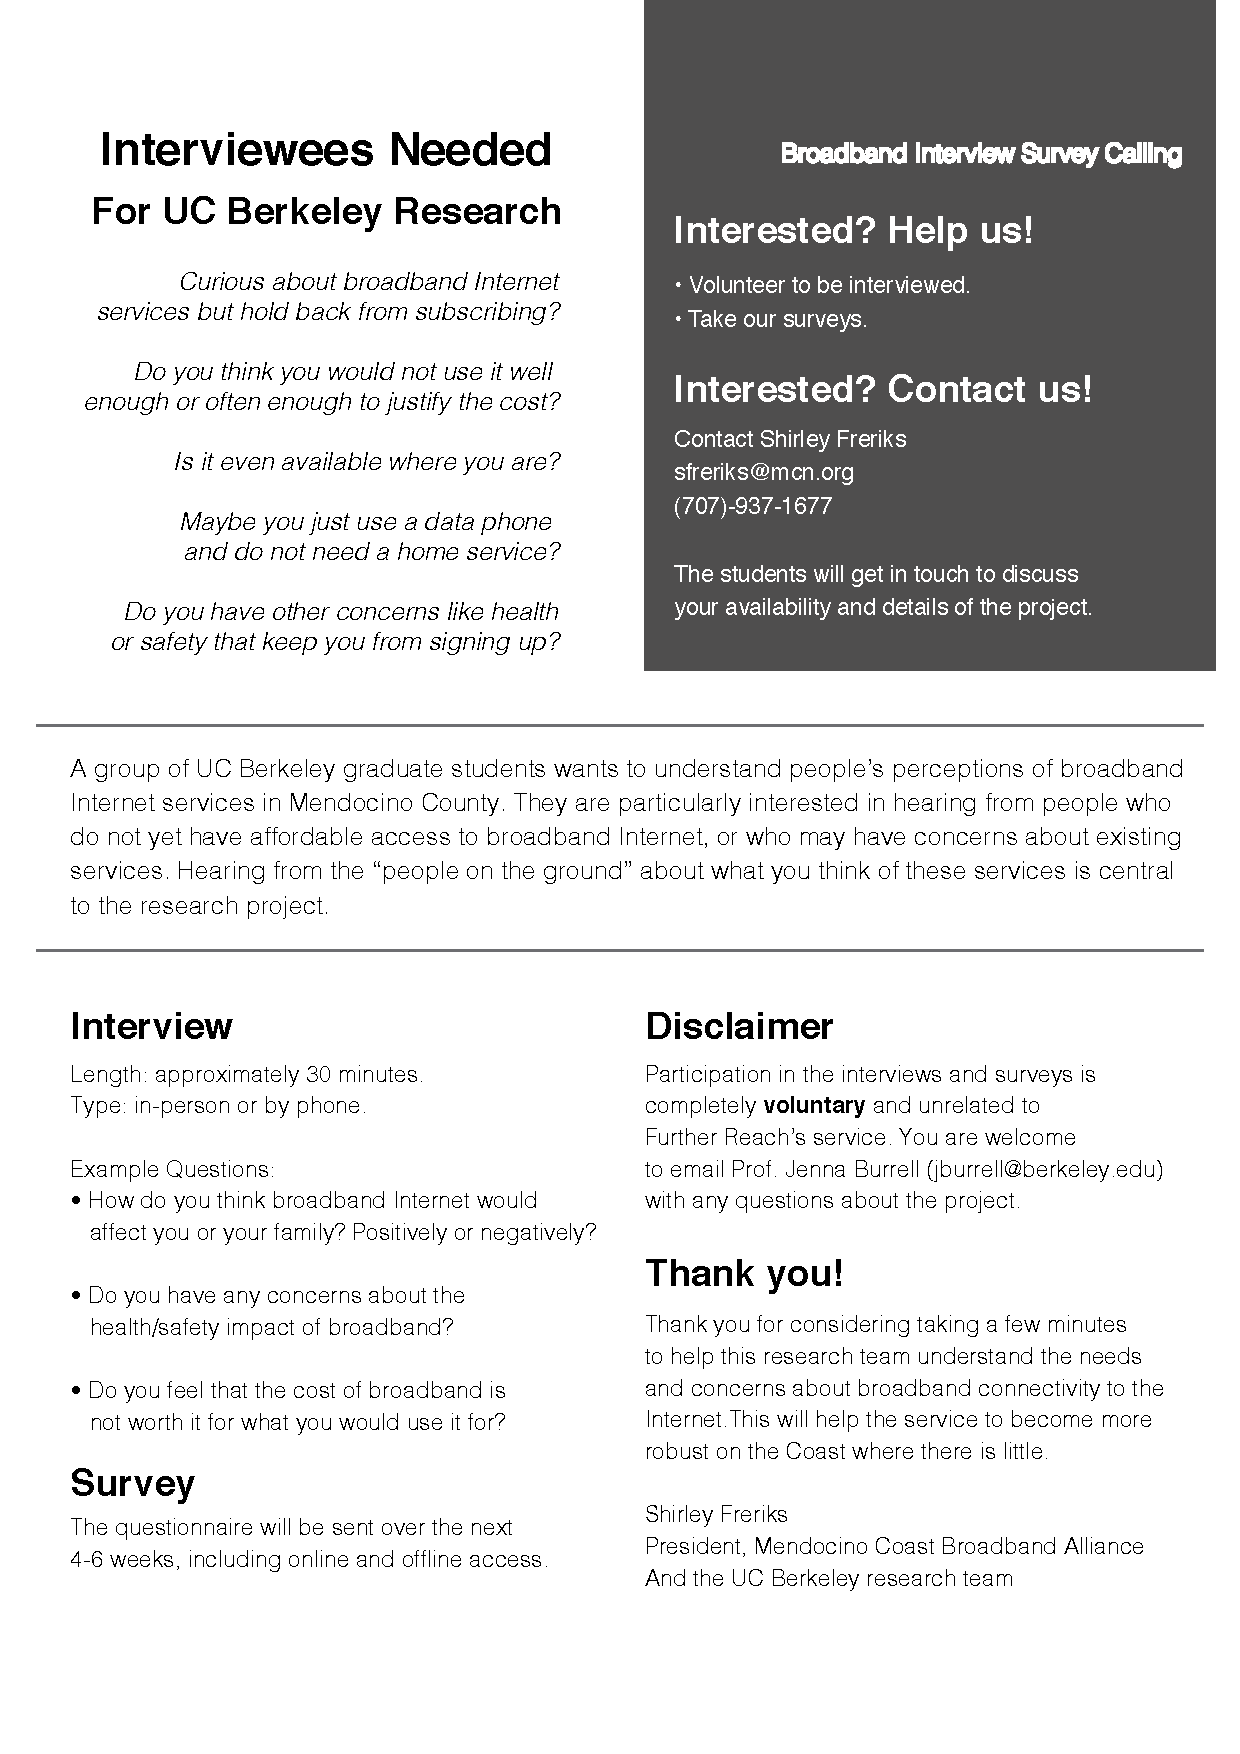
\includegraphics[scale=0.4]{../assets/flier-2.pdf}

\end{appendices}

\end{document}

%%% Local Variables:
%%% mode: latex
%%% TeX-master: t
%%% End:
